\documentclass[a4paper,dvipsnames]{article}

\input ../header
\newcommand{\checkedbox}{\makebox[0pt][l]{$\square$}\raisebox{.15ex}{\hspace{0.1em}$\checkmark$}}
\newcommand{\checkbox}{\makebox[0pt][l]{$\square$}\raisebox{.15ex}{\hspace{0.1em}}\hspace{3mm}}

\begin{document}

\title{Évaluation 4 -- Sujet A -- Éléments de correction}
\author{}
\date{}

\maketitle{}

\pagestyle{empty}

\exo\vspace{-2mm} 
\begin{enumerate}
  \item Écrire chaque nombre sous la forme $a\sqrt{b}$, où $a$ est un entier et $b$ l'entier naturel le plus petit possible.

    \begin{enumerate}
      \item {\color{red}$\sqrt{75}=\underbrace{\sqrt{25}}_{=5}\times\sqrt{3}=5\sqrt{3}$}
      \item {\color{red}$\sqrt{15}\times\sqrt{20}=\sqrt{300}=\sqrt{100}\times\sqrt{3}=10\sqrt{3}$}
      \item {\color{red}$3\sqrt{3}-2\sqrt{12}+\sqrt{300}=3\sqrt{3}-2\times\sqrt{4}\times\sqrt{3}+\sqrt{100}\times\sqrt{3}=3\sqrt{3}-4\sqrt{3}+10\sqrt{3}=9\sqrt{3}$}
    \end{enumerate}
  \item Écrire sans racine carrée au dénominateur :

    \begin{enumerate}
      \item {\color{red}$\dfrac{3}{\sqrt{7}}=\dfrac{3\sqrt{7}}{\sqrt{7}\times\sqrt{7}}=\dfrac{3\sqrt{7}}{7}$}
      \item {\color{red}$\dfrac{5}{\sqrt{6}-1}=\dfrac{5(\sqrt{6}+1)}{(\sqrt{6}-1)(\sqrt{6}+1)}=\dfrac{5(\sqrt{6}+1)}{5}=\sqrt{6}+1$}
    \end{enumerate} 

  \item Donner une valeur arrondie de $\dfrac{3}{\sqrt{7}}$ à $10^{-3}$ près, puis un encadrement d'amplitude $10^{-4}$ de $\dfrac{5}{\sqrt{6}-1}$.\\
    On obtient, grâce à la calculatrice, {\color{red}$\dfrac{3}{\sqrt{7}}\approx 1,134$} et {\color{red}$\np{3,4494}\leq \dfrac{5}{\sqrt{6}-1}\leq \np{3,4495}$}.
\end{enumerate}

\bigskip

\exo On fait tourner chacune des roulettes suivantes et on note la couleur obtenue. Modéliser chaque expérience aléatoire en complétant le tableau donné.

\begin{multicols}{2}
  \begin{center}
    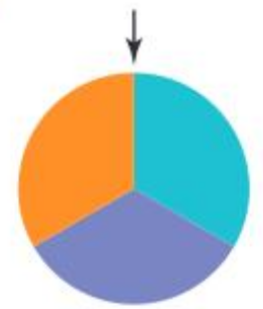
\includegraphics[width=2.5cm]{evaluation_4_figure_1.png}
  \end{center}

  \begin{center}
    \vspace*{0.7cm}
    \hspace*{-3cm}\begin{tabular}{@{}cccc@{}}
      \toprule
      Couleur obtenue & vert & orange & bleu\\
      \midrule
      Probabilité & {\color{red}$\dfrac{1}{3}$} & {\color{red}$\dfrac{1}{3}$} & {\color{red}$\dfrac{1}{3}$}\\
      \bottomrule
    \end{tabular}
  \end{center}
\end{multicols}

\begin{multicols}{2}
  \begin{center}
    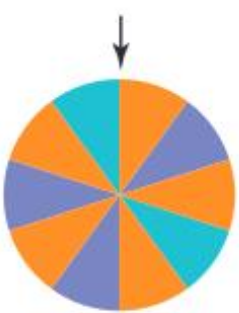
\includegraphics[width=2.3cm]{evaluation_4_figure_3.png}
  \end{center}

  \begin{center}
    \vspace*{0.75cm}
    \hspace*{-3cm}\begin{tabular}{@{}cccc@{}}
      \toprule
      Couleur obtenue & vert & orange & bleu\\
      \midrule
      Probabilité & {\color{red}$\dfrac{2}{10}$} & {\color{red}$\dfrac{5}{10}$} & {\color{red}$\dfrac{3}{10}$}\\
      \bottomrule
    \end{tabular}
  \end{center}
\end{multicols}

\bigskip

\exo On considère la fonction (incomplète) suivante écrite en Python :

\begin{minted}{python}
def mystere(B, b, h):
    a = ...
    return ...
\end{minted}

\begin{enumerate}
  \item Comment s'appelle cette fonction ?\\
    {\color{red}Cette fonction s'appelle \mintinline{python}{mystere}.}
  \item Combien de paramètres possède-t-elle ?\\
    {\color{red}Elle possède 3 paramètres.}
  \item Quel mot-clé permet de définir une fonction en Python ?\\
    {\color{red}Il s'agit du mot-clé \mintinline{python}{def}.}
  \item Compléter la fonction afin qu'elle renvoie l'aire d'un trapèze de bases $B$ et $b$, et de hauteur $h$.\\
    \textit{Remarque. -- On rappelle que l'aire d'un tel trapèze est donnée par la formule :
      \[\dfrac{(B + b)\times h}{2}.\]
  }
\begin{minted}{python}
def mystere(B, b, h):
    a = (B + b) * h / 2
    return a
\end{minted}
\item Comment utiliser cette fonction pour calculer l'aire d'un trapèze de bases $7$ et $5$, et de hauteur $3$ ?\\
  {\color{red}Il suffit d'écrire \mintinline{python}{mystere(7, 5, 3)}.}
\end{enumerate}

\end{document}
